
%(BEGIN_QUESTION)
% Copyright 2011, Tony R. Kuphaldt, released under the Creative Commons Attribution License (v 1.0)
% This means you may do almost anything with this work of mine, so long as you give me proper credit

An operator claims pressure gauge PG-108 is defective and needs to be replaced.  This pressure gauge registers 50 PSI, while pressure controller PIC-33 and pressure recorder PR-33 both register the pressure as being equal to setpoint: 43 PSI.  Before replacing this pressure gauge, however, you decide to do some diagnostic thinking to see if there might be other causes for the abnormally high reading at PG-108.  The first thing you check is the position of control valve PV-33a, and you find its stem position to be at 35\% open.  

$$\includegraphics[width=15.5cm]{i0001rx01.eps}$$

Identify the likelihood of each specified fault in this process.  Consider each fault one at a time (i.e. no coincidental faults), determining whether or not each fault could independently account for {\it all} measurements and symptoms in this process.

% No blank lines allowed between lines of an \halign structure!
% I use comments (%) instead, so that TeX doesn't choke.

$$\vbox{\offinterlineskip
\halign{\strut
\vrule \quad\hfil # \ \hfil & 
\vrule \quad\hfil # \ \hfil & 
\vrule \quad\hfil # \ \hfil \vrule \cr
\noalign{\hrule}
%
% First row
{\bf Fault} & {\bf Possible} & {\bf Impossible} \cr
%
\noalign{\hrule}
%
% Another row
PG-108 calibration error &  &  \cr
%
\noalign{\hrule}
%
% Another row
PT-33 calibration error &  &  \cr
%
\noalign{\hrule}
%
% Another row
PIC-33 left in manual mode &  &  \cr
%
\noalign{\hrule}
%
% Another row
PY-33a calibration error &  &  \cr
%
\noalign{\hrule}
%
% Another row
PY-33b calibration error &  &  \cr
%
\noalign{\hrule}
} % End of \halign 
}$$ % End of \vbox

Finally, identify the {\it next} diagnostic test or measurement you would make on this system.  Explain how the result(s) of this next test or measurement help further identify the location and/or nature of the fault.

\filbreak

\vskip 20pt \vbox{\hrule \hbox{\strut \vrule{} {\bf Suggestions for Socratic discussion} \vrule} \hrule}

\begin{itemize}
\item{} Based on the information you have at this point, can you tell whether any suspected calibration error is due to a mis-adjustment of {\it zero} or of {\it span}?  Explain why or why not.
\item{} Is controller PIC-33 direct-acting or reverse-acting?  How can you tell?
\item{} Does control valve PV-33a throttle gas or liquid?  How can you tell?
\item{} Identify a typographical error in this P\&ID.
\item{} A useful diagnostic technique for identifying which instrument is miscalibrated is to compare the readings of multiple instruments (all sensing the same process variable) to see which one of them disagrees mostwith the others.  May we apply this technique to the problem at hand?  If so, which instrument readings should we compare?  If not, explain why not.
\end{itemize}

\underbar{file i03512}
%(END_QUESTION)





%(BEGIN_ANSWER)

\noindent
{\bf Partial answer:}

% No blank lines allowed between lines of an \halign structure!
% I use comments (%) instead, so that TeX doesn't choke.

$$\vbox{\offinterlineskip
\halign{\strut
\vrule \quad\hfil # \ \hfil & 
\vrule \quad\hfil # \ \hfil & 
\vrule \quad\hfil # \ \hfil \vrule \cr
\noalign{\hrule}
%
% First row
{\bf Fault} & {\bf Possible} & {\bf Impossible} \cr
%
\noalign{\hrule}
%
% Another row
PG-108 calibration error &  &  \cr
%
\noalign{\hrule}
%
% Another row
PT-33 calibration error & $\surd$ &  \cr
%
\noalign{\hrule}
%
% Another row
PIC-33 left in manual mode &  &  \cr
%
\noalign{\hrule}
%
% Another row
PY-33a calibration error &  &  \cr
%
\noalign{\hrule}
%
% Another row
PY-33b calibration error &  &  \cr
%
\noalign{\hrule}
} % End of \halign 
}$$ % End of \vbox


%(END_ANSWER)





%(BEGIN_NOTES)

% No blank lines allowed between lines of an \halign structure!
% I use comments (%) instead, so that TeX doesn't choke.

$$\vbox{\offinterlineskip
\halign{\strut
\vrule \quad\hfil # \ \hfil & 
\vrule \quad\hfil # \ \hfil & 
\vrule \quad\hfil # \ \hfil \vrule \cr
\noalign{\hrule}
%
% First row
{\bf Fault} & {\bf Possible} & {\bf Impossible} \cr
%
\noalign{\hrule}
%
% Another row
PG-108 calibration error & $\surd$ &  \cr
%
\noalign{\hrule}
%
% Another row
PT-33 calibration error & $\surd$ &  \cr
%
\noalign{\hrule}
%
% Another row
PIC-33 left in manual mode &  & $\surd$ \cr
%
\noalign{\hrule}
%
% Another row
PY-33a calibration error &  & $\surd$ \cr
%
\noalign{\hrule}
%
% Another row
PY-33b calibration error &  & $\surd$ \cr
%
\noalign{\hrule}
} % End of \halign 
}$$ % End of \vbox


The fact that the gauge disagrees with both the recorder and the controller tells us the problem is either with the gauge, or with the transmitter.  Nothing else (controller mode, valve signal path, PY-33a) could cause this to happen.  Therefore, valid tests include anything to help is discern whether there is a problem in the gauge, in the transmitter, in the resistor, or in the controller's PV input.

\vskip 10pt

Try asking one or more of these questions to get the classroom session going:

\begin{itemize}
\item{} What would happen if someone loosened a tube fitting on the pneumatic output line of PT-33 with the pressure control loop in automatic mode?
\item{} What would happen if someone loosened a wire going to PY-33b with the pressure control loop in automatic mode?
\end{itemize}

















\filbreak \vskip 20pt \vbox{\hrule \hbox{\strut \vrule{} {\bf Virtual Troubleshooting} \vrule} \hrule}

\noindent
{\bf Predicting the effect of a given fault:} present each of the following faults to the students, one at a time, having them comment on all the effects each fault would produce.

\begin{itemize}
\item{} 
\item{} 
\item{} 
\end{itemize}


\vskip 10pt


\noindent
{\bf Identifying possible/impossible faults:} present symptoms to the students and then have them determine whether or not a series of suggested faults could account for all the symptoms, explaining {\it why} or {\it why not} for each proposed fault:

\begin{itemize}
\item{} Symptom: {\it }
\item{}  -- {\bf Yes/No}
\item{}  -- {\bf Yes/No}
\item{}  -- {\bf Yes/No}
\end{itemize}


\vskip 10pt


\noindent
{\bf Determining the utility of given diagnostic tests:} present symptoms to the students and then propose the following diagnostic tests one by one.  Students rate the value of each test, determining whether or not it would give useful information (i.e. tell us something we don't already know).  Students determine what different results for each test would indicate about the fault, if anything:

\begin{itemize}
\item{} Symptom: {\it }
\item{}  -- {\bf Yes/No}
\item{}  -- {\bf Yes/No}
\end{itemize}


\vskip 10pt


\noindent
{\bf Diagnosing a fault based on given symptoms:} imagine the ??? fails ??? in this system (don't reveal the fault to students!).  Present the operator's observation(s) to the students, have them consider possible faults and diagnostic strategies, and then tell them the results of tests they propose based on the following symptoms, until they have properly identified the nature and location of the fault:

\begin{itemize}
\item{} Operator observation: {\it }
\item{} 
\item{} 
\end{itemize}


%INDEX% Basics, control loop troubleshooting (realistic P&ID shown)
%INDEX% Measurement, pressure: troubleshooting
%INDEX% Process: distillation, generic (realistic P&ID shown)

%(END_NOTES)

